% this file is part of the Smart Card project.

% to-do
% -----
% - outline
% - write
% - submit
% - spend

\documentclass[letterpaper,12pt,preprint]{hack_aastex}
\usepackage{epsfig}
\usepackage{graphicx}
\newcommand{\sectionname}{Section}
\setlength{\headheight}{2ex}
\setlength{\headsep}{3ex}
%----- exact 1-in margins
% NB: headheight and headsep MUST exist and be set
\setlength{\textwidth}{6.5in}
\setlength{\textheight}{9in}
\addtolength{\textheight}{-1.0\headheight}
\addtolength{\textheight}{-1.0\headsep}
\setlength{\topmargin}{0.0in}
\setlength{\oddsidemargin}{0.0in}
\setlength{\evensidemargin}{0.0in}

%----- typeset certain kinds of words
\newcommand{\observatory}[1]{\textsl{#1}}
\newcommand{\package}[1]{\textsf{#1}}
\newcommand{\project}[1]{\package{#1}}
\newcommand{\an}{\package{Astrometry.net}}
\newcommand{\NASA}{\observatory{NASA}}
\newcommand{\Kepler}{\observatory{Kepler}}
\newcommand{\kepler}{\Kepler}
\newcommand{\MAST}{\observatory{MAST}}
\newcommand{\EA}{\observatory{Exoplanet Archive}}
\newcommand{\TESS}{\observatory{TESS}}
\newcommand{\galex}{\observatory{GALEX}}
\newcommand{\Spitzer}{\observatory{Spitzer}}
\newcommand{\gaia}{\observatory{Gaia}}
\newcommand{\lsst}{\observatory{LSST}}
\newcommand{\sdss}{\observatory{SDSS}}
\newcommand{\latin}[1]{\textit{#1}}
\newcommand{\eg}{\latin{e.g.}}
\newcommand{\etal}{\latin{et~al.}}
\newcommand{\etc}{\latin{etc.}}
\newcommand{\ie}{\latin{i.e.}}
\newcommand{\vs}{\latin{vs.}}

%----- typeset journals
% \newcommand{\aj}{Astron.\,J.}
% \newcommand{\apj}{Astrophys.\,J.}
% \newcommand{\apjl}{Astrophys.\,J.\,Lett.}
% \newcommand{\apjs}{Astrophys.\,J.\,Supp.\,Ser.}
% \newcommand{\mnras}{Mon.\,Not.\,Roy.\,Ast.\,Soc.}
% \newcommand{\aap}{Astron.\,\&~Astrophys.}

%----- Tighten up paragraphs and lists
\setlength{\parskip}{0.0ex}
\setlength{\parindent}{0.2in}
\renewenvironment{itemize}{\begin{list}{$\bullet$}{%
  \setlength{\topsep}{0.0ex}%
  \setlength{\parsep}{0.0ex}%
  \setlength{\partopsep}{0.0ex}%
  \setlength{\itemsep}{0.0ex}%
  \setlength{\leftmargin}{1.5\parindent}}}{\end{list}}
\newcounter{actr}
\renewenvironment{enumerate}{\begin{list}{\arabic{actr}.}{%
  \usecounter{actr}%
  \setlength{\topsep}{0.0ex}%
  \setlength{\parsep}{0.0ex}%
  \setlength{\partopsep}{0.0ex}%
  \setlength{\itemsep}{0.0ex}%
  \setlength{\leftmargin}{1.5\parindent}}}{\end{list}}

%----- mess with paragraph spacing!
\makeatletter
\renewcommand\paragraph{\@startsection{paragraph}{4}{\z@}%
                                    {1ex}%
                                    {-1em}%
                                    {\normalfont\normalsize\bfseries}}
\makeatother

%----- Special Hogg list for references
  \newcommand{\hogglist}{%
    \rightmargin=0in
    \leftmargin=0.25in
    \topsep=0ex
    \partopsep=0pt
    \itemsep=0ex
    \parsep=0pt
    \itemindent=-1.0\leftmargin
    \listparindent=\leftmargin
    \settowidth{\labelsep}{~}
    \usecounter{enumi}
  }

%----- side-to-side figure macro
%------- make numbers add up to 94%
 \newlength{\figurewidth}
 \newlength{\captionwidth}
 \newcommand{\ssfigure}[3]{%
   \setlength{\figurewidth}{#2\textwidth}
   \setlength{\captionwidth}{\textwidth}
   \addtolength{\captionwidth}{-\figurewidth}
   \addtolength{\captionwidth}{-0.02\figurewidth}
   \begin{figure}[htb]%
   \begin{tabular}{cc}%
     \begin{minipage}[c]{\figurewidth}%
       \resizebox{\figurewidth}{!}{\includegraphics{#1}}%
     \end{minipage} &%
     \begin{minipage}[c]{\captionwidth}%
       \textsf{\caption[]{\footnotesize {#3}}}%
     \end{minipage}%
   \end{tabular}%
   \end{figure}}

%----- top-bottom figure macro
 \newlength{\figureheight}
 \setlength{\figureheight}{0.75\textheight}
 \newcommand{\tbfigure}[2]{%
   \begin{figure}[htp]%
   \resizebox{\textwidth}{!}{\includegraphics{#1}}%
   \textsf{\caption[]{\footnotesize {#2}}}%
   \end{figure}}

%----- deal with pdf page-size stupidity
\special{papersize=8.5in,11in}
\setlength{\pdfpageheight}{\paperheight}
\setlength{\pdfpagewidth}{\paperwidth}

% no more bad lines!
\sloppy

\newcommand{\kplr}{\package{kplr}}
\newcommand{\Untrendy}{\package{Untrendy}}
\newcommand{\Turnstile}{\package{IronHorse}}
\newcommand{\Bart}{\package{Bart}}
\newcommand{\emcee}{\package{emcee}}
\newcommand{\TheCreator}{\package{TheCreator}}
\newcommand{\KIC}{\textsl{KIC}}
\newcommand{\KOI}{\textsl{KOI}}
\pagestyle{myheadings}
\markright{\textsf{\small Hogg \& Foreman-Mackey / probabilistic modeling of Kepler data}}

\usepackage{color,listings}
\lstset{%
    language=Python,
    basicstyle=\footnotesize\ttfamily,
    showspaces=false,
    showstringspaces=false,
    tabsize=2,
    breaklines=false,
    breakatwhitespace=true,
    identifierstyle=\ttfamily,
    keywordstyle=\bfseries\color[rgb]{0.133,0.545,0.133},
    commentstyle=\color[rgb]{0.4,0.4,0.4},
    stringstyle=\color[rgb]{0.627,0.126,0.941},
}

\begin{document}

\section{why re-analyze \Kepler\ data?}

The \Kepler\ team is one of the most successful collaborations in the
history of astronomy, and the \Kepler\ data are by no means trivial to
understand and use.  Why would even a plucky twosome consider
competing with this extremely capable group?  The answer is that this
is \emph{not} a proposal to \emph{compete} with the \Kepler\ team.
This is a proposal to enhance the capabilities of the \Kepler\ mission
and give new tools to the entire community to increase the scientific
return from the \Kepler\ data (and many related and future data sets).

The first reason that it makes sense to re-consider the \Kepler\ data
from the ground up is the simple point that it is valuable to have
multiple eyes on the problem.  We bring different prejudices,
different intuitions, and different expertise than exists on the
\Kepler\ team.  In addition, we can analyze the \Kepler\ data in a
more open-ended way since we do not bear the responsibility of
delivering results according to existing schedules and requirements.
That said, we very much hope to create methods and code that make the
\Kepler\ team products more valuable and easier to deliver.

The second reason it makes sense for us to take an independent look at
the \Kepler\ data is that we will bring a strong probabilistic,
causal, generative model approach to everything we do.  In each
component of this project, we are trying to write down a probability
for the data given the parameters, and in each component we are trying
to have the relationship of the parameters to the predictions obey
deep ideas we have about the physical or causal processes that
generate the data.  For certain kinds of (endearing) fanatics---or
perhaps more correctly, under certain kinds of restrictive
assumptions---these probabilistic approaches to data analysis are
guaranteed to succeed over more heuristic methods.  We have god on our
side, in this sense.  But because we are free from project
requirements, we can take a more principled approach to the data
analysis and see if that delivers better results.  If it does (because
we are proposing to generate public, open-source, easy-to-use code)
\emph{everybody wins.}

Finally, the most important reason to bring new people and new ideas
to the \Kepler\ data is that the \Kepler\ data are so damned
important.  The vast majority of known exoplanets are
\Kepler\ discoveries (CITE), and each \Kepler\ discovery brings with
it so much important information about each planetary system (CITE).
The data set has included many multiple-planet systems, and supported
preliminary studies of population statistics, such as multiplicity and
inclination distributions (CITE).  These studies have been made
possible in part by the scale and in part by the simplicity of the
\Kepler\ experiment; it has created a statistically useable sample.
Although \Kepler\ is just the first step of \NASA's exoplanet journey,
it is the best data set in it's class right now, and will retain
unique capabilities for many years to come.  Furthermore, many future
data sets (for example that from \TESS; CITE), produce data that are
\Kepler-like in many ways.  \textbf{If we can take the most valuable
  data set in exoplanetary astrophysics and make it substantially more
  valuable with an ADAP-scale project, we can deliver to
  \NASA\ outstanding science per dollar.}

Even if you are convinced that the data need to be re-analyzed, why
should they be reanalyzed by this team?  Although the proposers do not
have a long history in exoplanet science, we do have some experience,
breaking ground in the area of hierarchical modeling of exoplanet
populations (CITE Hogg), and telescope light-field modeling for
exoplanet direct detection and spectroscopy (CITE Oppenheimer).  Much
more importantly, the proposal team has enormous experience in two
areas that are crucial if we are going to squeeze more information out
of the \Kepler\ data stream: We have great experience with calibration
and sensitive statistical analysis of enormous astrophysical data
sests (CITE some eg papers), and we are among the world leaders in
probabilistic modeling of astrophysical data sets (CITE some eg
papers).  In particular, Co-I Hogg was partially responsible for the
precise self-calibration of the \observatory{Sloan Digital Sky Survey}
imaging data (CITE Padmanabhan), which in turn led (almost directly)
to discoveries such as ultra-faint Milky Way companions Willman I
(CITE) and XXX (CITE) and the detection of the baryon acoustic feature
in the large-scale structure (CITE).  These two
strengths---calibration and probabilistic modeling---are not unique to
the proposing team, but their combination is unusual and puts us in a
very strong position to deliver extremely valuable new methods to the
\Kepler\ team and larger community.

\section{tools for easy access to \Kepler\ data}

\paragraph{Sources of \Kepler\ data}
The official source of Kepler data is the Mikulski Archive for Space
Telescopes (MAST) archive.
MAST also includes complete catalogs of stellar parameters, \Kepler\ Object of
Interest (KOI) parameters, and the measured parameters of confirmed planets
in the \Kepler\ field.
Another catalog of exoplanet parameters is the NASA Exoplanet Archive%
\footnote{http://exoplanetarchive.ipac.caltech.edu/}.
The Exoplanet Archive hosts a complete mirror of the MAST \Kepler\ tables but
it also includes results from other exoplanet studies.
The standard method for accessing data from these catalogs is through at web
form%
\footnote{http://archive.stsci.edu/kepler/data\_search/search.php}%
\footnote{http://exoplanetarchive.ipac.caltech.edu/applications/ExoTables%
/upload.html}
but both services also offer programmatic access via an Application
Programming Interface (API).
This is especially interesting to these authors because we are interested in
doing automated data analysis.
It is also generally useful to have easy access to data from a standard
scientific programming environment because it lets an interested user apply
their standard analysis tools to new datasets easily.
In general, all programming languages that are commonly used for science have
libraries designed to interact with web services using HTTP requests so it's
possible to access the \Kepler\ data from any language.
That being said, these tools tend to be very general so for any particular
query that you would like to make, you'll need to construct the URL by hand
and then parse the returned text using a custom set of tools.
This can be time consuming and tends to be error prone so many users will
resort to using the HTML web form and downloading and importing the data by
hand.
This can be a significant obstacle for the development of automated data
analyses.

Maybe comment on JSON.\


\paragraph{\kplr\ interface}
We propose to build a library to easy data access directly from the Python
programming environment.
Python is a good choice for this for several reasons.
First, many astronomers are beginning to adopt Python as their main
programming language (CITE dotastro?) and there are many powerful
astronomy-specific tools that are becoming part of the standard scientific
stack---especially \package{AstroPy} (http://www.astropy.org/).
Also, Python has many tools---such as \package{iPython} (http://ipython.org/)
and the \package{iPython} notebook (http://ipython.org/notebook.html)---for
interactive data exploration.
The proposed interface should satisfy at least the following requirements:
\begin{itemize}
\item The interface should be general enough that any request that could
possibly be made from the web form should be possible.
\item Common tasks (like searching for a particular planet or the top 10
largest KOIs, for example) should be easy.
\item The results should be automatically parsed into a Python object with the
correct types so that it can be easily integrated with existing tools.
\item The results syntax should be consistent for different data types.
\end{itemize}
Below is an example of the proposed syntax for the module.
This code could be run from the interactive Python prompt or from within a
script.

\begin{lstlisting}
import kplr
client = kplr.API()

# Get the listing for the confirmed planet Kepler-10 b
kepler10b = client.planet("10b")
print(kepler10b)
# <kplr.Planet("Kepler-10 b")>

print(kepler10b.period)
# 0.8374903

# Loop over available datasets and download the light curves from MAST.
for d in kepler10b.data:
    d.fetch()
    # ...
    # Analyse the dataset using d.time, d.sapflux, etc.
    # Plot using matplotlib or whatever.

# Find the 10 largest KOIs.
kois = client.kois(sort=("planet_radius", -1), limit=10)
\end{lstlisting}

The development on this tool has started on GitHub at
https://github.com/dfm/kplr and a pre-release version is already available
under the liberal MIT open source license.


\section{de-trending}

Key features of \project{untrendy}:
\begin{itemize}
\item Very scalable/local compared to ``Bayesian'' algorithm. Similar to
      a more robust windowed median.
\item Finds discontinuities---called Sudden Pixel Sensitivity Dropouts (SPSD)
      by the Kepler team---automatically and corrects the trends. There is a
      claim in the literature (with reference to a non-existent
      Kolodziejczak 2012 paper) that PDC in the Kepler pipeline 8.0 will deal
      with this but it's not included as part of the standard de-trending.
\item Untrendy is probably less robust to maintaining intrinsic stellar
      variability but if the goal is a \emph{planet search} then something
      scalable that removes any non-planetary signal is interesting.
\end{itemize}

\paragraph{Standard Pre-search Data Conditioning (PDC)}
The first step in the Kepler plant search is to remove systematic trends in
the data.
Transit signals can be significantly diluted by both intrinsic stellar
variability and instrumental effects. In general, these features can be much
larger than the transit signals so care must be taken to separate
blah blah Sudden Pixel Sensitivity Dropouts (SPSDs)

\paragraph{Standard Practice}
For most precision experiments, the light curves corrected using PDC are not
sufficiently de-trended.
It is standard practice (Dressing, for example) to normalize fluxes by a
running windowed median with a width of a few days (this is a free parameter).
This method actually works very well.
It corrects for most of the smooth systematic signals and can remove any
stellar variability on time scales longer than the window width.
Using the median is extremely robust to outliers so if you use a wide enough
window, this procedure doesn't significantly affect the transit signal.
It is important to note that if you're looking to study the parameters of the
\emph{planets} it is often preferable to remove the effects of stellar
variability.
It would probably not be a good idea to do something as simplistic as a
windowed median if you're interested in studying the properties of variable
stars.
This procedure runs into serious trouble when it encounters a SPSD or any
other sharp discontinuity.
The implicit background model must be smooth even across discontinuities so it
will introduce significant structured residuals at SPSDs.
The most responsible procedure would probably be to simply discard the data
near these points (as with PDC) but the literature is not very clear on how
this is done in practice.


\paragraph{``Bayesian'' MAP-PDC}
\begin{itemize}
\item uses co-trending with surrounding stars to remove systematic trends that
\emph{are correlated} between nearby sources.
\item should also deal with SPSDs (word on the street) but the paper doesn't
exist.
\item this will be included in the ``next'' official release of the Kepler
pipeline but it hasn't been yet so we can't compare.
\item this is probably FAR better for studies of variable stars.
\item the other side of the same coin is that it probably isn't as good for
studying planets unless your model of the star includes a model of stellar
variability\ldots and if you're going to that trouble, why aren't you forward
modelling the systematics too.
\item also, if you're trying to \emph{find} exoplanets, a more destructive
algorithm is probably better suited.
\end{itemize}


\paragraph{Untrendy}
Our algorithm and implementation---currently titled \Untrendy---takes a
somewhat different approach.
Using only a single quarter of data as input, the algorithm will attempt to
remove all systematic variations (and properly account for SPSDs) while
maintaining the strength of any existing transit signal.
Initial experiments have produced extremely promising results even when
reproducing the lowest signal-to-noise discoveries in the Kepler catalog.

The proposed algorithm involves an iterative procedure with two distinct
steps.
The first step fits a cubic spline model (with one knot every few days; will
probably work best for denser sampling than the median filter model) using
iteratively re-weighted least-squares (IRLS;\ Hogg: some sort of citation?) to
the median normalized aperture photometry.
Then, discontinuities can be detected using a matched filter on the residuals
from the model fit in the previous step.
Finally, after adding $K$ knots in the discontinuity, return to the first IRLS
step and repeat.

IRLS is a good choice for this purpose because it is extremely robust to
outliers.
This means that it can fit and correct for the global trends but not corrupt
the transit signal.
The optimization will also be insensitive to the outliers caused by the
discontinuities until the model is given more flexibility (in the form of
added knots) at these positions.

The choice of a cubic spline model with iteratively chosen knots is
justified---and preferable to a windowed median model---for several reasons.
First, it is significantly simpler (in general) that the median or PDC models.
The number of free parameters in the model is only the total number of knots
in the spline.
Contrast this to the median model (and probably the PDC model\ldots who
knows?) where the model implicitly has the same number of parameters as
data points.
Also, the spline model can have variable complexity (or flexibility) at
different points---a fact that we are taking advantage of to correct for
discontinuities.
Furthermore, spline models can be evaluated extremely efficiently so a model
like the one that we propose here is not significantly more computationally
complex than a median filter model.

We propose to release a implementation of this algorithm as a standalone C
library with Python bindings under a liberal open source license (MIT!).
This algorithm could be easily incorporated into any analysis where a running
median is currently in use.
It would also be a complimentary addition to the standard Kepler data
product along side the PDC and MAP-PDC results.


\paragraph{Enhanced goals}
While the data pre-processing algorithm described above is a realistic and
quickly obtainable first step towards better modeling and detection of
exoplanets in the Kepler data stream, it leaves the probabilistically
righteous among us a little unsatisfied.
The cubic spline model suggested above is only a very rough approximation to
the physical (causal) model that we have of the data and by applying this
point estimated model we introduce significantly correlated noise and don't
correctly propagate the uncertainty introduced by the modeling procedure.
An exiting prospect for improving this procedure would be to model the data
using a flexible non-parametric probabilistic model like a Gaussian Process
 (CITE STUFF).
Applying a Gaussian process to a dataset as large as a Kepler light curve is
an interesting problem in computer science but since most of the power in the
systematics is at short time lag, it would be possible to take advantage of
the sparsity of the problem for efficiency (Iain Murray?).

Another interesting idea would be to---like the MAP-PDC algorithm does---take
advantage of correlations between the systematic variations of nearby sources.
In particular, a qualitative study of the some Kepler targets has shown that
the locations of discontinuities tend to be the same for sources that are
nearby on the detector.

What about near periodicity in the systematic trends between quarters?


\begin{figure}[p]
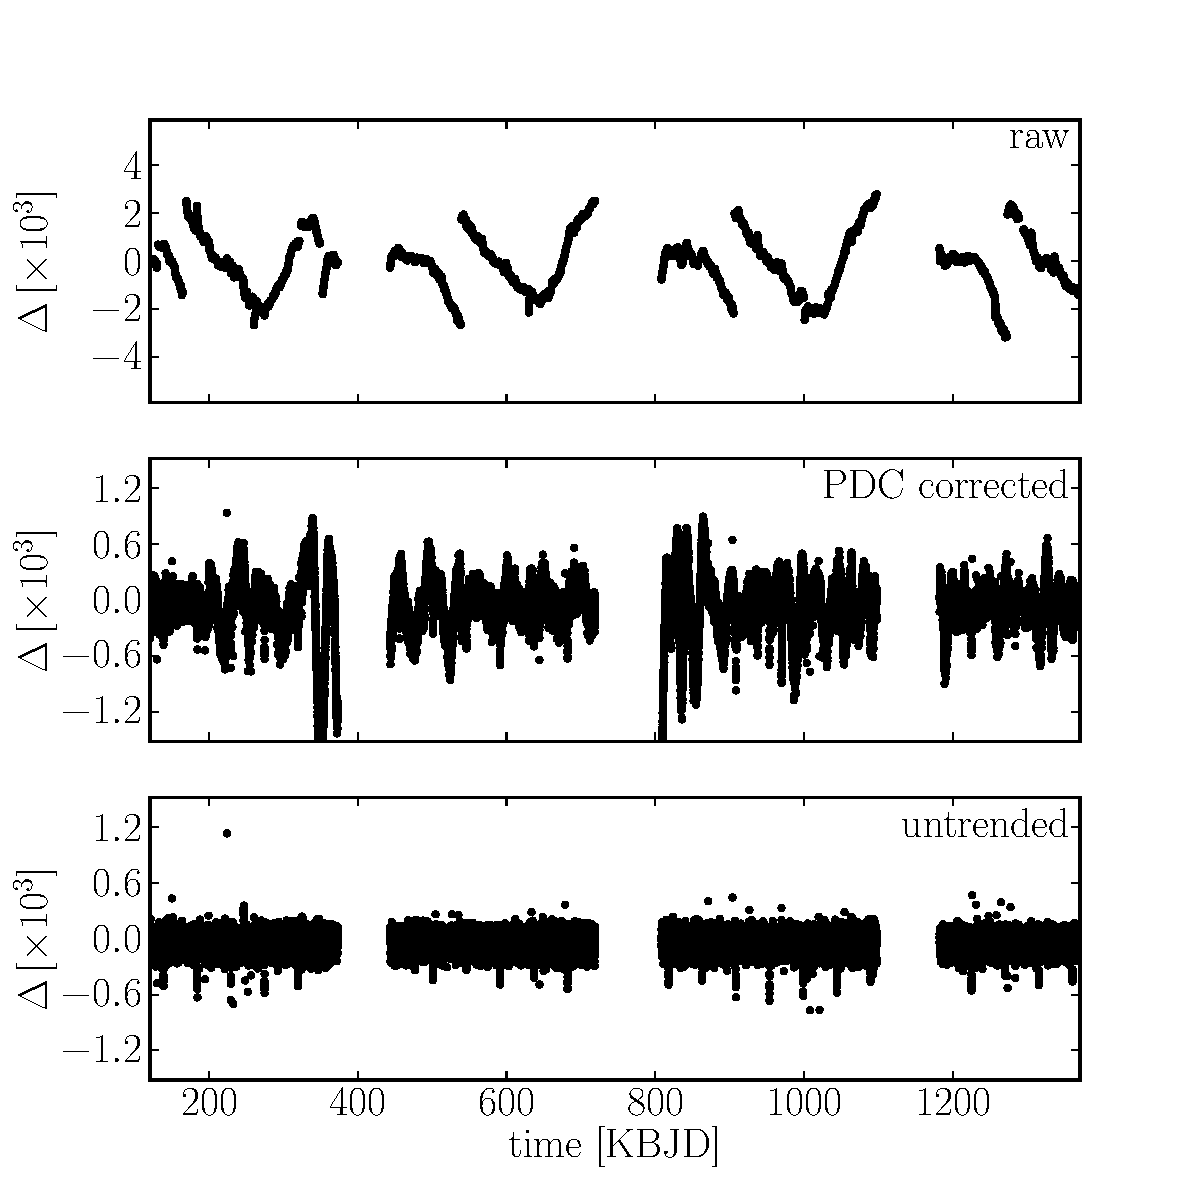
\includegraphics[width=\textwidth]{figures/untrend_data.pdf}
\caption{%
The long cadence observations of the star Kepler-10.
There are two confirmed exoplanets in this system.
\emph{Top:} the raw aperture photometry from the Kepler data reduction
pipeline.
For plotting purposes, each quarter was normalized by the median flux in the
quarter and then 1 was subtracted to show the variation around the median.
\emph{Middle:} the PDC corrected fluxes.
Again, the fluxes were normalized by the median and then shifted to zero
median.
Note the change of units on the y-axis; the PDC procedure clearly makes good
progress towards removing the main systematic trends in the data.
\emph{Bottom:} the light curve after untrending.
The units on the y-axis are the same as the middle panel.
The results are way better\ldots WAY.
\label{fig:untrendy}}
\end{figure}

\section{fast, approximate hypothesis testing}

DFM:  Explain what is currently done and how.  With citations.

Hogg:  Explain what \Turnstile\ will do in its first release.

DFM:  And demo figure.

Hogg:  Explain what future releases of \Turnstile\ might do.


\section{probabilistic parameter estimation}

Main features of \Bart:
\begin{itemize}
\item Flexible, non-parametric limb-darkening profile.
\item Fast standalone Fortran library.
\item User-friendly Python bindings with expressive model-building syntax.
\item Efficient sampling using \emcee \citep{emcee}.
\end{itemize}

\paragraph{Current practice for parameter estimation}
\citet{mandel}

\paragraph{Enhanced goals}
False positive detection using LD discrepancies.


\section{hierarchical population inference}

...pgm intro

...DFM:  Explain what is currently done, perhaps concentrating on Tremaine
paper and competitors.  Also we should touch on theory here.

...Hogg:  What will \TheCreator\ do?

\section{side projects}

...GALEX project

...false-positive detection and characterization

...variable-star science

\section{management plan}

This project is the PhD dissertation project of Co-I Foreman-Mackey;
in this sense Foreman-Mackey is the scientific lead of the project,
making decisions about scientific priorities and the ordering of
experiments and code enhancements.  PI Hogg is the faculty advisor on
this dissertation; in this sense Hogg is the management lead of the
project, ensuring that deadlines get met, papers get written, and code
gets properly documented and released.  The budget also includes a
small amount of support for an additional part-time graduate student
and postdoc.  These are budgeted to support short-term scentific
collaborations that make use of the software or improve it.  That is,
some of the sub-parts of the project can be executed by new graduate
students or postdocs at NYU.

The project is budgeted for three years of project lifetime.  An
approximate schedule is the following

\paragraph{first year:}
Complete and release version~1.0 of \kplr\ API.  Release version~0.1
of \Untrendy, \Turnstile, and \Bart, executing the first stages of
approximation identified above.  Submit short papers describing these
codes, comparing them with standard community practice, and showing
first results.  Execute \Untrendy\ and \Turnstile\ on the entire \KIC;
publication of all candidate transiting exoplanets, especially those
previously unknown.  Execute \Bart\ on the best or most interesting of
those companions, with an eye to exoplanet characterization and
false-positive rejection.

\paragraph{second year:}
Submit papers describing the results of the \Untrendy, \Turnstile, and
\Bart\ from the first year.  Complete and release version~0.1 of
\TheCreator, executing the simplest meaningful graphical model, as
described above.  Execute \Bart\ and \TheCreator\ on the complete set
of exoplanet candidates geenerated in the first year.  Submit paper
describing those results.  With feedback from this full ``closed
loop'', re-prioritize enhancements to \Untrendy\ and \Turnstile; add
features to \Bart.  Complete and release Version~0.2 code for these
packages.  Start side projects on stellar variability, eclipsing
binaries, transit-timing variations, or limb-darkening as appropriate.

\paragraph{third year:}
Following up best hints in results from \TheCreator\ in the second
year, complexify or adjust the graphical model, or launch multiple
models for competition.  Re-run everything on the entire \KIC\ to
update the population analysis to incorporate all improvements.
Submit papers describing improved software and new results.  Complete
side projects and submit papers.  Make final decisions about final
code versions, final code adjustments, documentation, and hosting and
release Version~1.0 for all four of \Untrendy, \Turnstile, \Bart, and
\TheCreator, along with (possibly very short) papers on arXiv or ASCL.

\begin{thebibliography}{}\raggedright%

\bibitem[Foreman-Mackey \etal(2012)]{emcee}
Foreman-Mackey, D., Hogg, D.~W., Lang, D., \& Goodman, J.\ 2013,
\pasp, \textbf{125}, 306

\bibitem[Mandel \& Agol(2002)]{mandel}
Mandel, K., \& Agol, E.\ 2002, \apjl, \textbf{580}, L171

\end{thebibliography}

\end{document}
